\subsection{Simplifying the model}
I will need to make many assumptions when modelling the landing of the aeroplane. This is because, it can be very difficult and complex to take into account every little detail, therefore by making a few assumptions, I will be able to model the landing of the plane without making the model too complex and also keeping the model feasible to work with.

\subsubsection{Assumptions Made and their relevance to the situation:}

\textbf{Aeroplane:} 
\begin{enumerate}
    \item The plane acts as a point
    If we did not take the plane to act as a particle, then the equations formed would be extremely complex. By taking the plane to act as a particle, we do not need to take into account the shape of the plane, which in turn means we can ignore the rotational forces and also do not need to bother about how the air particles flow above the plane. Also we would not need to take into account the aerodynamics of the plane, which can over-complicate our model. Therefore, by we will assume that the plane acts as a particle.
    
    \item The mass of the aeroplane does not change
    If the mass of the plane change then we would not be able to use the special case of Newtons second Law, i.e $F=ma$, instead we would need to use the general law, which states that force is the rate of change of momentum. This would however, over-complicate our model, therefore i have decided that i will be assuming that the mass of the plane does not change.
\end{enumerate}
\
\textbf{Runway:}
\begin{enumerate}
  
  \item Runway is made out of the same material of all the way through
  If the runway was not made out of the same material, all the way through, then we would need to consider the friction between the wheels and the runway for each different material that the runs on. I addition to this, we would also need to split out model into multiple different cases for each different material the aeroplane drives on.
  
  \item The runway is smooth and flat
  If the landing was not flat, it would mean that we would need to consider all the different bumps there are across the runway. This is because, there bumps can have an impact on the velocity of the plane. Furthermore, if the runway had holes, then that would also have an impact on the velocity of the plane, thus it is best if we assume that the landing is smooth and flat.
\end{enumerate}
\
\textbf{Landing:} 
\begin{enumerate}
    \item Landing is completely straight
    If the landing was not straight, then that would mean that the friction would increase for the tires, meaning that the force change that occurred would need to be considered making the equations much more complex.
    
\end{enumerate}
\
\textbf{Weather:} 
\begin{enumerate}
    \item No wind speed on the ground
    If there was wind speed on the ground, depending upon which direction the wind is moving, it could result in an increased air resistance or a decreased air resistance. This would affect our equations greatly and we would need to consider the force the wind exerts on the plane. This would be extremely complex as we would also need to model the wind speed, which is extremely complicated
    
    \item Weather conditions do not change
    If the weather conditions changed, it would mean that the air resistance would also change. Depending upon how the air resistance changes, the air Resistance could increase or decrease. If the temperature of the air increased, it would mean that the air became less dense, meaning that the air resistance has decreased. The converse is also true, as in if the temperature decreased, it would result in increased air resistance as the plane hits more air particles.
    
    \item The air resistance is constant
    For our initial model, I am assuming that air resistant is constant. Although, I am assuming that air resistance is constant, we may change this assumption depending upon how our model performs against the data.
    
\end{enumerate}

\subsubsection{Importance}
Finally, the assumptions in their respective order of importance, as in which assumption would have the greatest impact on the model are:
\begin{enumerate}
    \item The plane acts as a point
    \item Weather conditions do not change
    \item No wind speed on the ground
    \item The runway is smooth and flat
    \item The mass of the aeroplane does not change
    \item Runway is made out of the same material of all the way through
    \item Landing is completely straight
    \item The air resistance is constant
\end{enumerate}

\subsubsection{Relevance of Assumptions}
Using the assumptions that the runway is completely level and smooth we know that the plane does not accelerate in the vertical direction. This means that both the forces, weight and normal reaction, are equal in magnitude. Therefore, from this it is clear that we will only need to model the velocity in the horizontal direction only.

Furthermore, the only force that is acting in the horizontal direction, before the breaks have been applied, is the force of air resistance. This means that the only force that needs to be considered when modelling the velocity of the plane before the breaks have been applied is the force of air resistance. However, once the breaks have been applied, we will need to take into the breaking force as well as the force of air resistance. By taking both forces into account, we will be able to model the situation once the breaks have been applied until the aeroplane has come to a stop.

Here are the force diagrams that represent our model subject to the assumptions made.

\begin{figure}[H]
    \centering
    \subfloat[Case 1 - Before $F_b$ applied] {{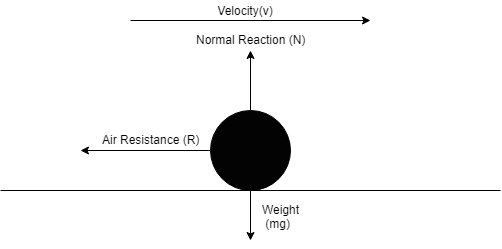
\includegraphics[width=7cm]{Introduction/ModelDiagrams/Case1.png}}}
    \qquad
    \subfloat[label 2 - After $F_b$ applied] {{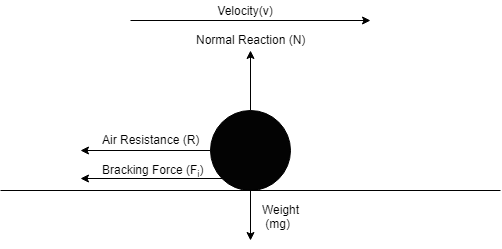
\includegraphics[width=7cm]{Introduction/ModelDiagrams/Case2.png}}}
    \caption{Modelling the Aeroplane as a point particle}
    \label{fig:example}
\end{figure}